\section{The dataset}
\label{chapter2_section3}

The dataset of the project is designed to be consistent with the large macro dataset used in the dynamic factor model of \cite{Giannone2008}. It comprises a series of quarterly real GDP for the United States, which represents the main target to predict. Besides GDP, the nowcasts are realised from a set of 31 monthly variables for the United States, covering different sides of economic activity. The dataset is organised over seven blocks: general business indicators, production and sales, labor and wages, macroeconomic aggregates, prices, money and credits, interest rates and finance. All the series come from standard public sources such as the OECD, the Federal Reserve, or the Saint Louis FRED database. The details of the series are provided in Figure \ref{fig_c2_s3_1}.

\begin{figure}[H]
\centering
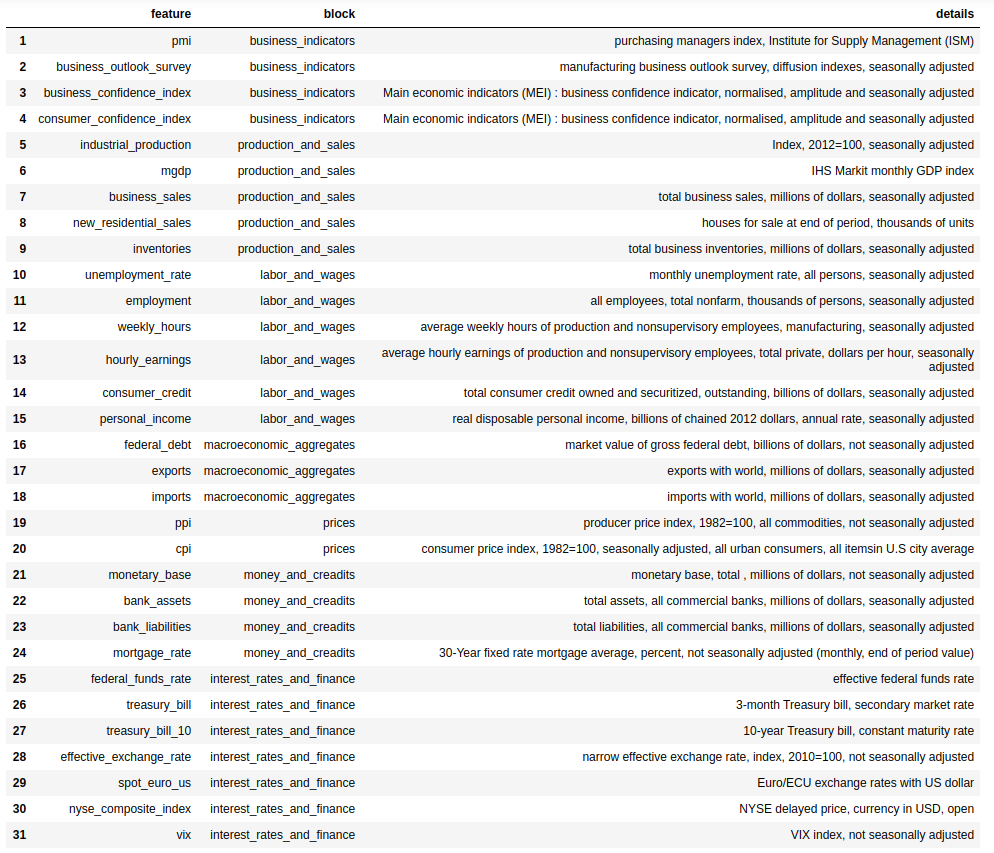
\includegraphics[scale=0.62]{images/information_dataframe.png}
\caption{Details of the monthly features used in the project}
\label{fig_c2_s3_1}
\end{figure}

This dataset calls for a few comments. First, the raw data is typically non-stationary. It must thus be differenced before being used within a time-series or machine learning framework. Following the recommandations of \cite{Giannone2008}, three possible transformations are applied. These transformations are detailed in Table \ref{table_c2_s3_1}.

\newpage

\begin{table}[H] \centering
\scalebox{0.9}{ \begin{tabular}{@{} lll @{}}
\toprule[0.5mm]
& Transformation & Description  \\
\cmidrule{1-3}
1 & $x_{i,t} = (1 - L^3) (1 + L + L^2) X_{i,t}$ & quaterly difference \\
2 & $x_{i,t} = (1 - L^3) (1 + L + L^2) log(X_{i,t}) \times 100$ & quarterly growth rate \\
3 & $x_{i,t} = (1 - L^3) (1 + L + L^2) (1 - L^{12}) log(X_{i,t}) \times 100$ & quarterly difference of yearly growth rate \vspace{2mm} \\
\bottomrule[0.5mm]
\end{tabular}}
\captionsetup{justification=centering}
\caption{\textbf{Raw data transformations}}
\label{table_c2_s3_1}
\end{table}

These transformations serve two purposes: stationarize the data, and formulate monthly values as quarterly quantities. This way, monthly estimates become comparable with the quarterly values of the real GDP series. The transformation applied to each specific series (along with the source of the data series) are reported in Appendix \ref{appendix2}. An overview of the transformed series is provided in Figure \ref{fig_c2_s3_2}. 

Second, due to the availability of certain data series, the sample only covers the period from 1993 to 2019. This represents a monthly sample of size 320. While this is usually fine for nowcasting and econometrics models, it is usually insufficient for machine learning methods which are extremely data greedy and requires several thousands of observations to properly learn the possible non-linearities in the data. The latter are thus clearly at a structural disadvantage here. The choice to end the sample in 2019 is explicit. Because of the recent COVID pandemy, the world economy collapsed brutally in 2020 so that the data for this year represents a huge outlier. Preliminary estimates with the COVID year proved quite abnormal and sometimes displayed aberrent behaviours. While predicting economic behaviours in a time of changing environment is a question with an interest on its own, it is not the purpose of the present project. As a consequence, it seemed safer to exclude 2020 from the sample to keep only regular behaviours, at least for now.

\newpage

\begin{figure}[H]
\centering
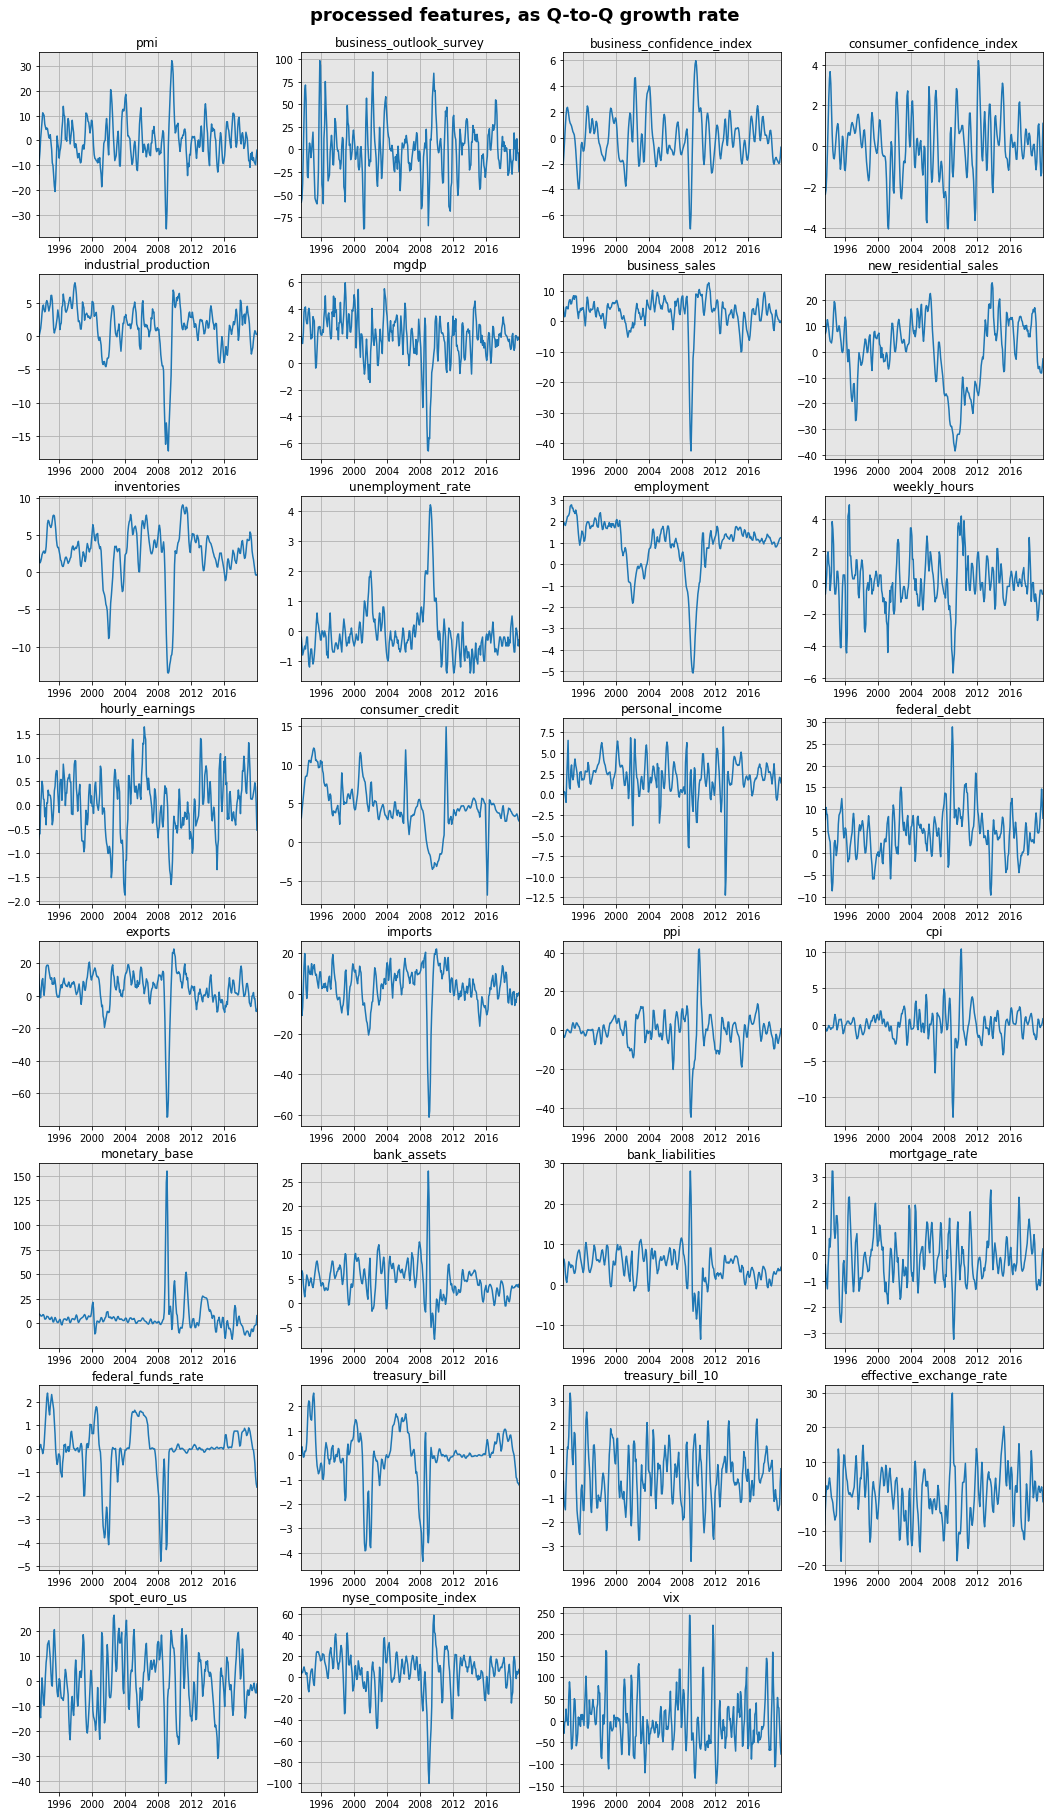
\includegraphics[scale=0.36]{images/processed_features.png}
\caption{Processed features}
\label{fig_c2_s3_2}
\end{figure}

Third and finally, the dataset was sometimes adapted to fit a given model. Most econometrics and machine learning models for instance can only handle single frequency data. In this case, the dataset had to be reduced to a quarterly dataset, omitting two out of three months in the original monthly set to keep only the months were quarterly releases occur. This reduces the sample size to just over 100, which represents a very short sample. Also, the full dataset of 31 variables does not seem suitable for all models. While certain methodologies like the dynamic factor model or the random forest usually perform best with a large dataset, other methods like the VAR model perform better with a dozen of feature or so (see for instance \cite{Giannone2015} for a discussion on the predictive performance of large VAR model). As a consequence, and to keep the exercise fair to all the models considered, a smaller dataset was created as a subset of the original dataset. This small dataset comprises only 9 monthy features (in addition to quarterly GDP), which are detailed in Figure \ref{fig_c2_s3_3}.

\begin{figure}[H]
\centering
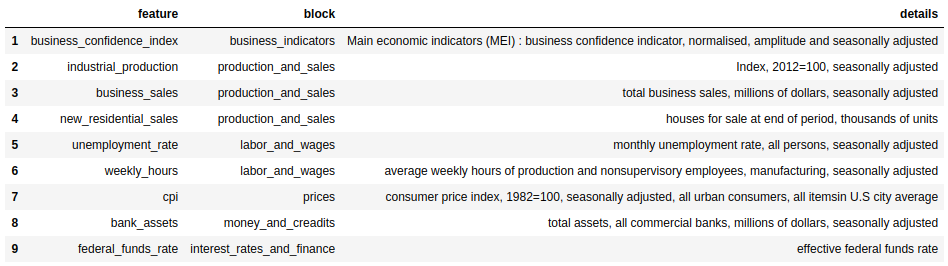
\includegraphics[scale=0.63]{images/small_dataset_dataframe.png}
\caption{Features included in the reduced dataset}
\label{fig_c2_s3_3}
\end{figure}





















